\subsection{Registradores}

Registradores são estruturas de memória compostas por múltiplos flip-flops.

\begin{figure}[H]
    \centering
    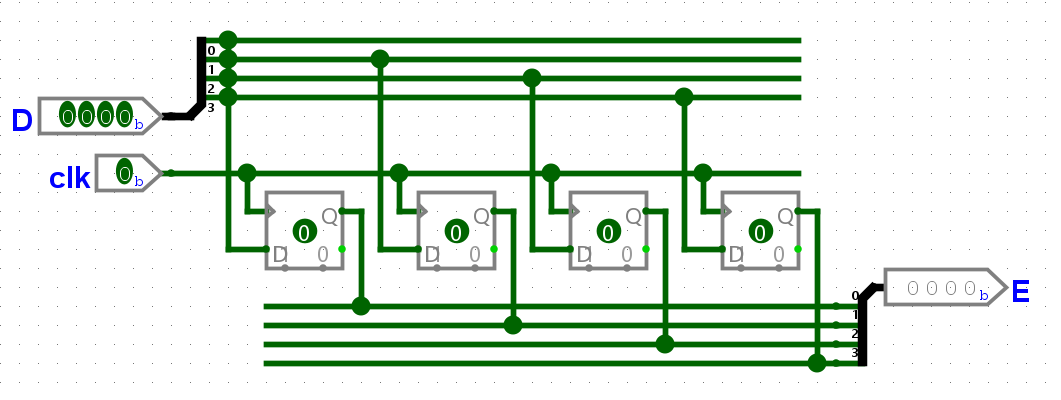
\includegraphics[width=0.8\linewidth]{images/D-Reg-4bit.png}
    \caption{Registrador de 4 bits Utilizando flip flops tipo D}
    \label{fig:D-Reg-4bit}
\end{figure}

Um registrador de $n$ bits armazena um estado $Q$ em um vetor:

\[
Q = (Q_0, Q_1, ..., Q_{n-1})
\]

De tal forma que todos os bits $Q_i \forall i \in [0, n-1]$ são atualizados simultaneamente no pulso de clock.

Esse será um componente fundamental para este projeto, visto que o estado do cronômetro, será armazenado em registradores a base de flip flops tipo D.